\documentclass{beamer}
\mode<presentation>
\usepackage{tikz}
\usepackage{graphicx}
\usepackage{tabu}
\usetikzlibrary{positioning}
\usetikzlibrary{calc}
\usetikzlibrary{backgrounds}
\usefonttheme{professionalfonts}
\usetheme{Orr}
\usepackage[orientation=portrait,width=42in,height=42in,scale=1.4]{beamerposter}
\usepackage{fontawesome}
\usepackage{xintexpr}
\usepackage{calculator}
\graphicspath{{./figures/}{./figures/generated/}{./figures/static/}}

\title{Reference-free Base Quality Score Recalibration for Sensitive Detection of Mutations}
\titlegraphic{
	
\includegraphics[width=.95\linewidth]{biodesign_logo.pdf}
	}
\date{3/22/19}
\author{Adam J Orr \inst{1,2} \faTwitter @AdamJOrr}
\institute{\inst{1} School of Life Sciences, Arizona State University \\
		   \inst{2} Biodesign Institute, Arizona State University}
\email{\faEnvelopeO \space ajorr1@asu.edu}
\website{\faLink \space   cartwrig.ht/lab/}

\begin{document}

\begin{frame}{}
\begin{columns}

%%%% Left side %%%%

\column{.5\linewidth}

%%%%%%%%%%%%%%%%%%%

% \begin{block}{\large Abstract}
% DNA sequencing and methods that use the resulting sequencing data to detect genetic variation play an important role in many studies. Associated with the sequencing data are quality scores, which measure the probability of technical error at each base in the sequence. Statistical models for detecting variants utilize these scores to determine which sequences are reliable and which are not. However, these scores are often poorly calibrated and underestimate the probability of error, causing overconfidence in the results. Base quality score recalibration is a process to increase the accuracy of quality scores, which leads to more accurate inferences. However, current methods for base quality score recalibration require a reference genome and are inaccurate if the quality of the reference is poor. We present a reference-free method for base quality score recalibration which performs similarly to previous methods but can be used without a reference.
% \end{block}


\begin{block}{Introduction}

\begin{itemize}
\item Illumina sequencing reads contain errors
\item Errors make mutation detection difficult
\item Quality scores represent $P(error)$ on a phred scale.
\begin{displaymath}
P(error) = 10^{\frac{-Q}{10}}
\end{displaymath}
\begin{displaymath}
Q = -10\log_{10}{P(error)}
\end{displaymath}
\item Though quality scores can be any integer, to reduce the size of data files they are sometimes binned into \textbf{7} bins 
\end{itemize}
\end{block}

\begin{block}{Base Quality Score Recalibration - BQSR}
Base Quality Score Recalibration is a technique to undo binning \textit{and} improve calibration of the original quality scores.
However, \textbf{BQSR requires a reference genome and a database of variable sites}. This is done using the \texttt{lighter} software,
which inspects the kmer spectrum to find erroneous bases rather than comparing the sequence to the reference.

\begin{figure}
\begin{center}

\textbf{GATK BQSR - Reference Required}

\begin{tikzpicture}[framed, align=center, sqnode/.style={rectangle,draw=black!60,fill=black!5,very thick,minimum size=1cm}, node distance = 4 cm]
	\node[sqnode] (sequencing) {Sequence};
	\node[sqnode] (alignment) [right = of sequencing] {Alignment};
	\node[sqnode] (ignorevar) [right = of alignment] {Ignore Variable Sites};
	\node[sqnode] (lookupref) [below = 2cm of alignment] {Assume Reference Mismatches Are Errors};
	\node[sqnode] (lnmodel) [below = 2cm of lookupref] {Predict Error Rate with Linear Model};
	\draw[line width=3mm,->] (sequencing) -- (alignment);
	\draw[line width=3mm,->] (alignment) -- (ignorevar);
	\draw[line width=3mm,->] (ignorevar) -- (lookupref);
	\draw[line width=3mm,->] (lookupref) -- (lnmodel);
\end{tikzpicture}
\end{center}
\end{figure}

\begin{figure}
\begin{center}

\textbf{Reference Free BQSR}

\begin{tikzpicture}[framed, align=center, sqnode/.style={rectangle,draw=black!60,fill=black!5,very thick,minimum size=1cm}, node distance = 4 cm]
	\node[sqnode] (sequencing) {Sequence};
	\node[sqnode] (kmer) [below = 2cm of sequencing] {Inspect Kmer Spectrum to Find Erroneous Bases with \texttt{lighter}};
	\node[sqnode] (lnmodel) [below = 2cm of kmer] {Predict Error Rate with Linear Model};
	\draw[line width=3mm,->] (sequencing) -- (kmer);
	\draw[line width=3mm,->] (kmer) -- (lnmodel);
\end{tikzpicture}

\end{center}
\end{figure}

\end{block}

\begin{block}{Hierarchical Linear Model}

The recalibration uses a hierarchical linear model to predict the true probability of error given a set of covariates.
Each covariate causes the predicted quality score to shift up or down from the predicted score one level above it in the hierarchy.

The relevant covariates are:
\begin{itemize}
	\item Read Group
	\item Original Assigned Quality Score
	\item Position in read and whether read is forward or reverse (Cycle)
	\item Base called and the prior base call (Context)
\end{itemize}

\begin{figure}
\begin{center}

\textbf{Hierarchical Linear Model}

\begin{tikzpicture}[align=center, sqnode/.style={rectangle,draw=black!60,fill=black!5,very thick,minimum size=1cm}, node distance = 4 cm]
	\node[sqnode,align=center,above,minimum size=16cm](rg) at (8,0){};
	% \draw[help lines] (0,0) grid (16,16);
	\node[](rglab) at (8,15){Read Group};
	\node[sqnode, align=center,above,minimum size=13cm,fill=gold!10](q) at (8,1){};
	\node[](qlab) at (8,12){Assigned Quality Score};
	\node[sqnode, minimum size = 5 cm,fill=maroon!10] at (5,6) {Cycle};
	\node[sqnode, minimum size = 5 cm,fill=maroon!10] at (11,6) {Context};
\end{tikzpicture}
\end{center}
\end{figure}

If 

\end{block}

% \begin{block}{Methods: Variant Detection}

% 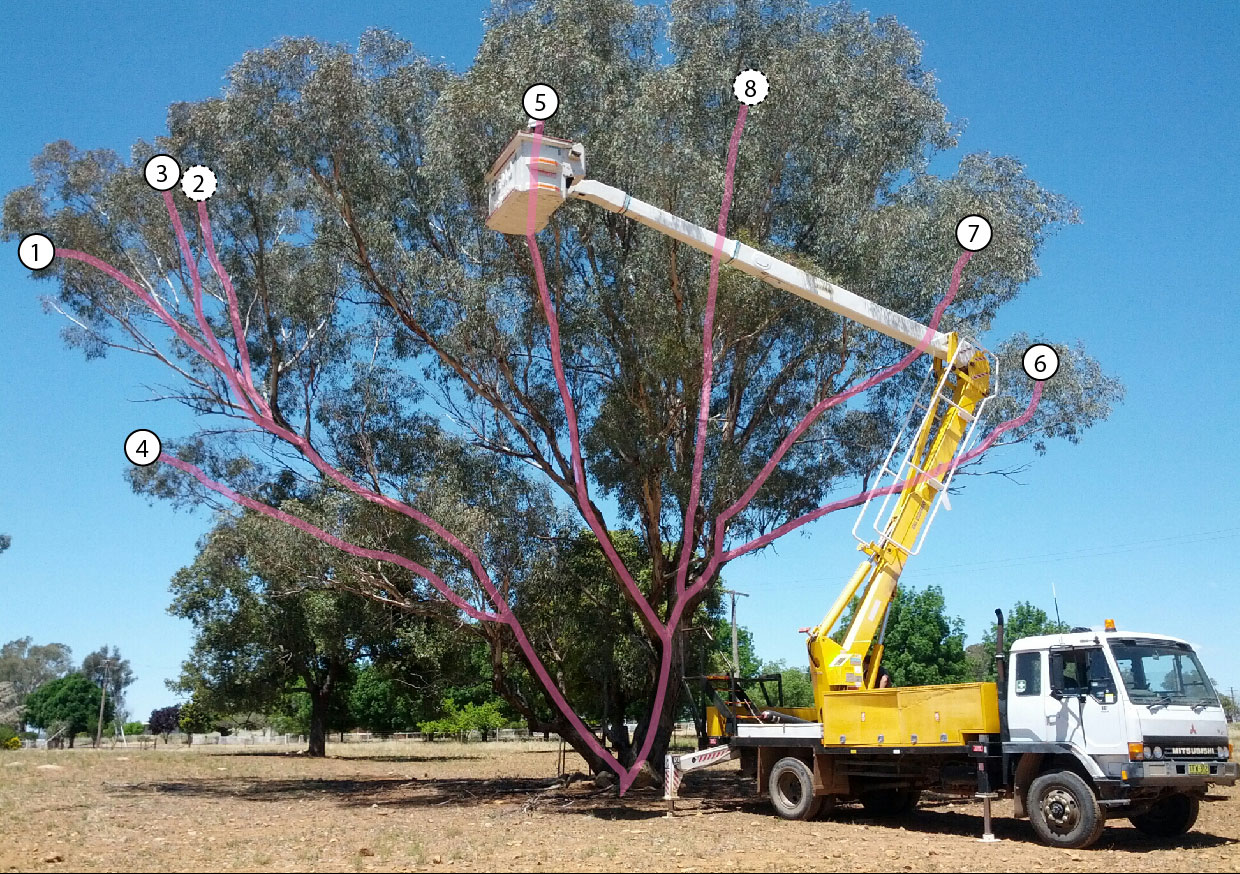
\includegraphics[width=.97\linewidth]{labeled_tree.jpg}

% \vskip 2ex

% \begin{itemize}
% \item 8 samples collected in triplicate
% % \item Each replicate was Illumina sequenced
% % \item Each sequence was aligned to genome of \textit{Eucalyptus grandis} using bwa mem.
% % \item Variants were called using GATK's UnifiedGenotyper or DiscoSNP++, a reference-free variant caller
% % \item Nonvariable sites and gaps were removed
% \item Variants were removed if the genotypes of all replicates of a sample were not identical
% % \item A maximum likelihood tree was constructed with RAxML
% \end{itemize}

% \vskip 2ex

% \begin{center}
% 	\begin{tikzpicture}[align=center, sqnode/.style={rectangle,draw=black!60,fill=black!5,very thick,minimum size=1cm}]
% 		\node[sqnode] (sequencing) {Sequence};
% 		\node[sqnode] (filter) [below = 7cm of sequencing] {Filter};
% 		\node[sqnode] (alignment) [below left = of sequencing] {Alignment};
% 		\node[sqnode] (gatk) [above left = of filter] {Get Variants (GATK)};
% 		\node[sqnode] (discosnp) [above right = of filter] {Get Variants (DiscoSNP++)};
% 		\node[sqnode] (tree) [below = of filter] {Tree Construction};
% 		\draw[line width=3mm,->] (sequencing) -- (alignment);
% 		\draw[line width=3mm,->] (sequencing) -- (discosnp);
% 		\draw[line width=3mm,->] (alignment) -- (gatk);
% 		\draw[line width=3mm,->] (gatk) -- (filter);
% 		\draw[line width=3mm,->] (discosnp) -- (filter);
% 		\draw[line width=3mm,->] (filter) -- (tree);
% 	\end{tikzpicture}
% \end{center}


% \end{block}

% \begin{block}{Results: Variant Detection}

% \vskip 1ex

% % \begin{columns}
% % 	\column{.4\linewidth}
% % 	\begin{block}{GATK}
% % 	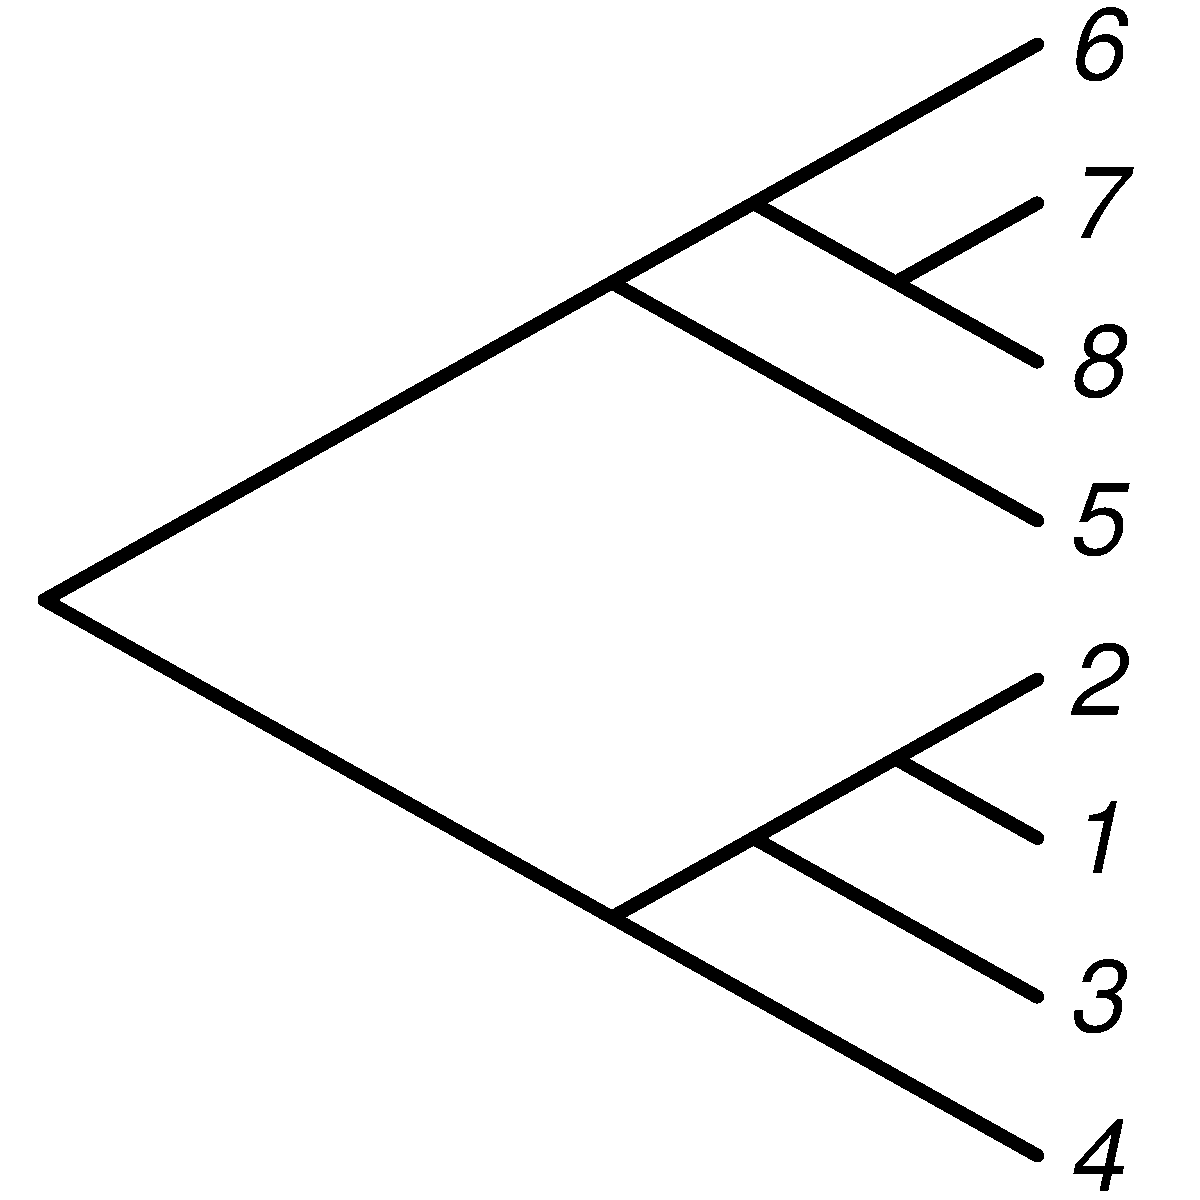
\includegraphics[width=.95\linewidth]{gatk_tree_rightwards.pdf}
% % 	\end{block}
% % 	\begin{block}{DiscoSNP++}
% % 	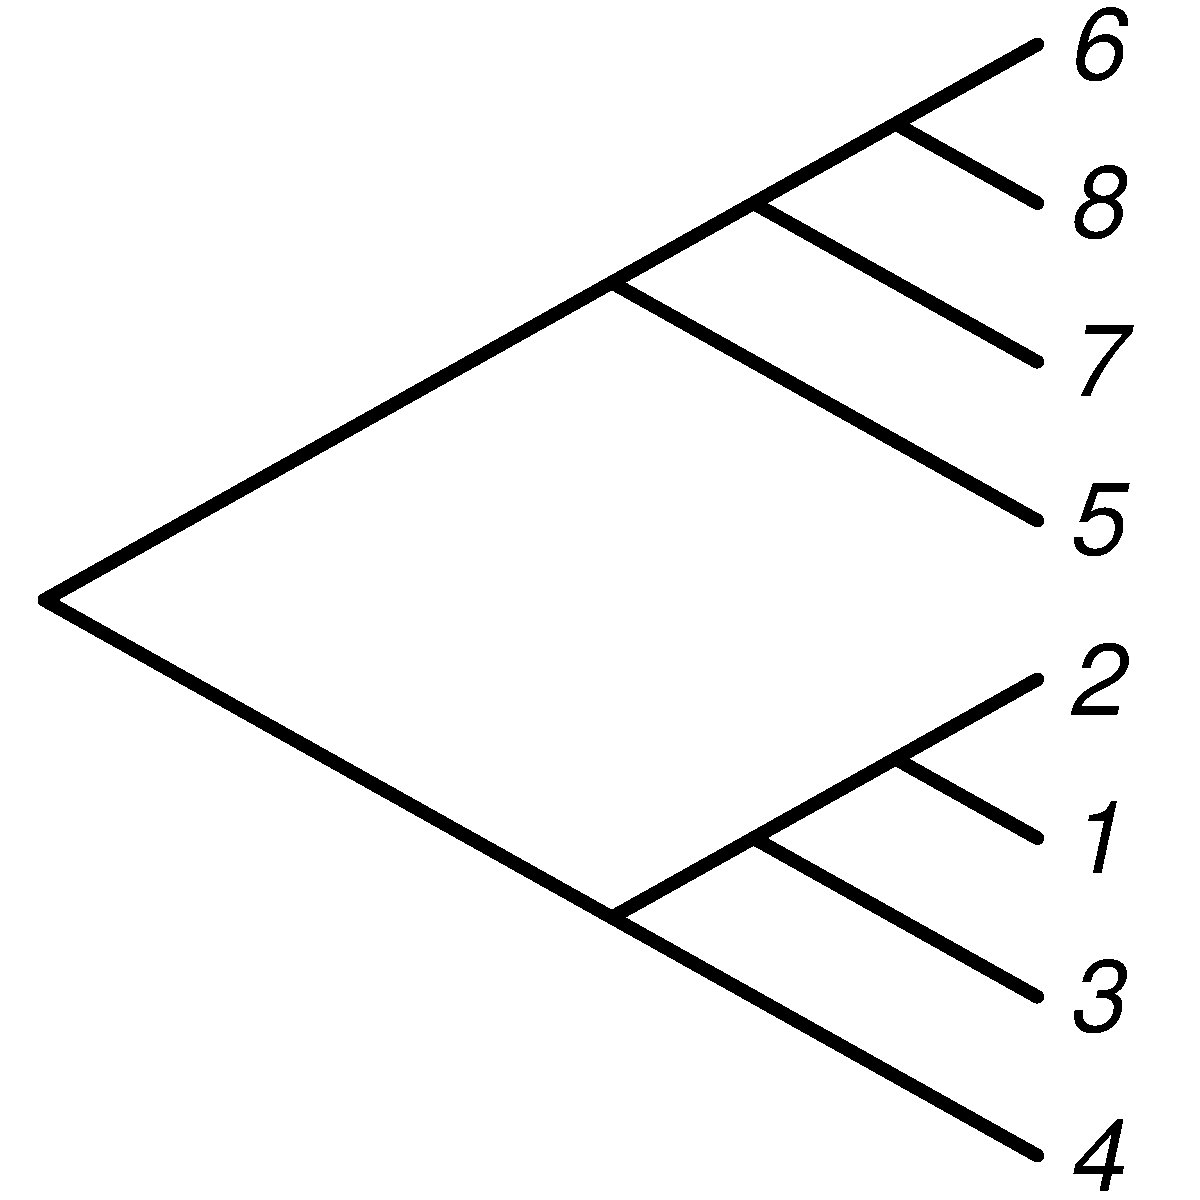
\includegraphics[width=.95\linewidth]{disco_tree_rightwards.pdf}
% % 	\end{block}
% % 	\column{.4\linewidth}
% % 	\begin{block}{True Topology}
% % 	\begin{center}
% % 	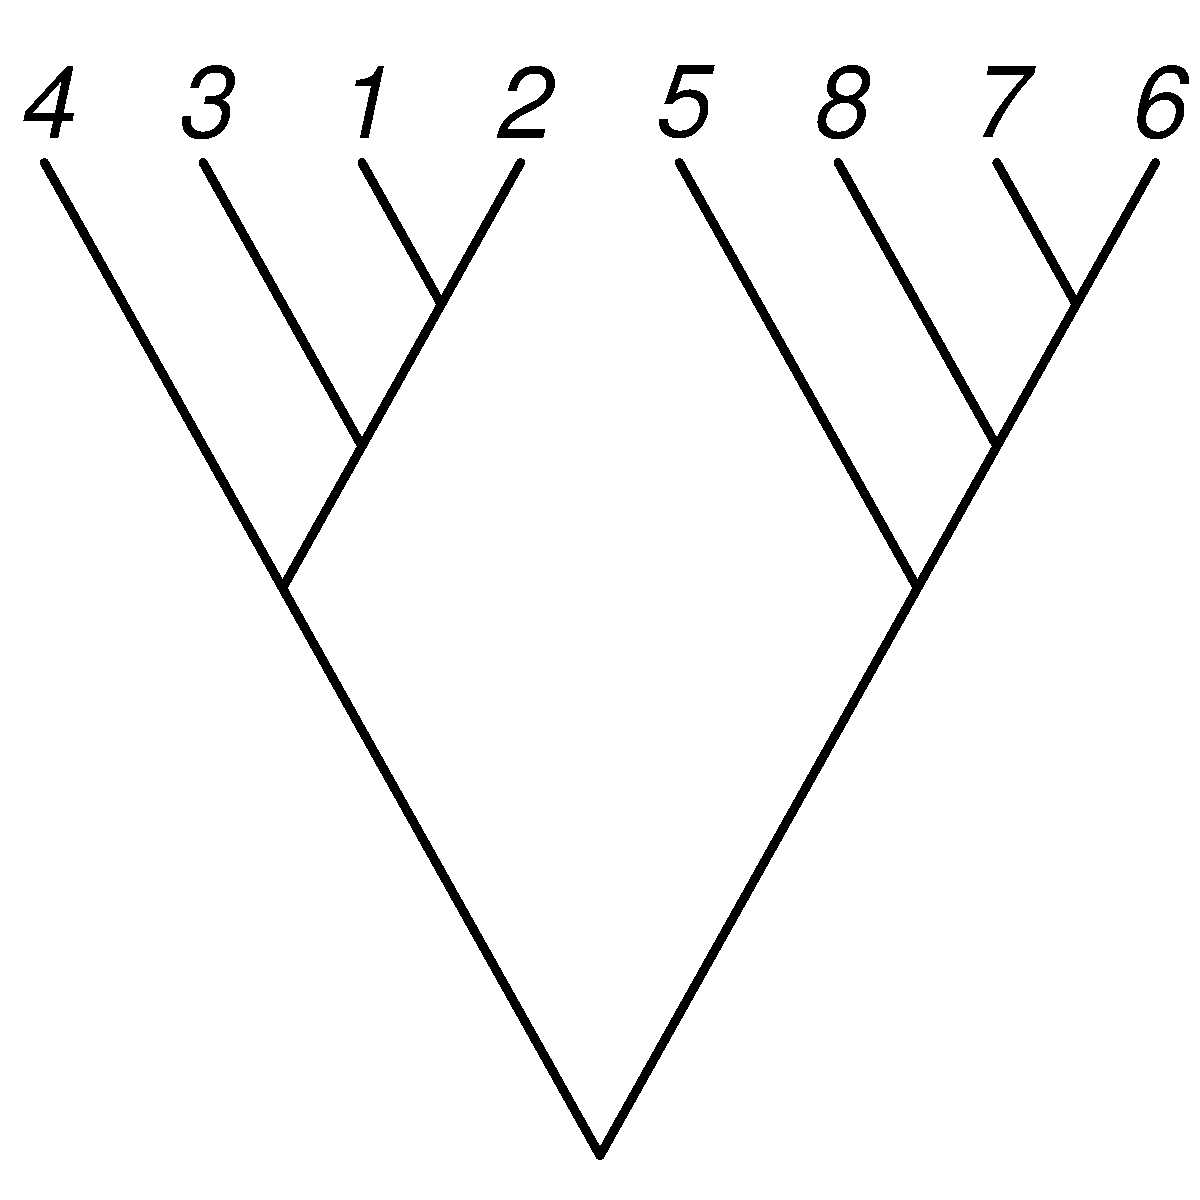
\includegraphics[width=.95\linewidth,angle=90]{true_tree.pdf}
% % 	\vskip 1ex
% % 	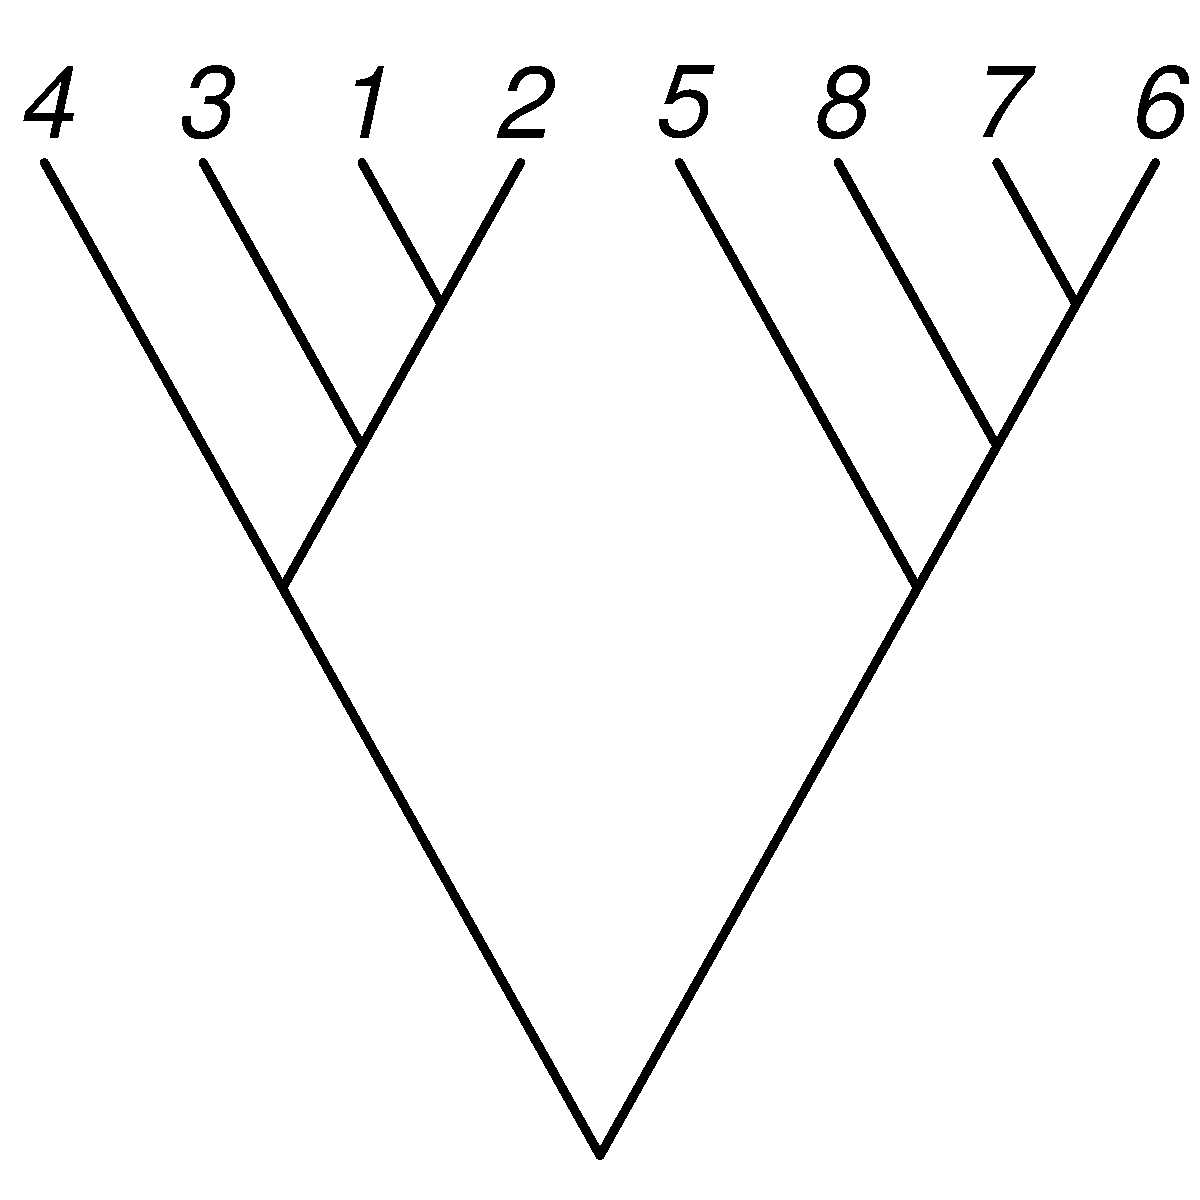
\includegraphics[width=.95\linewidth,angle=90]{true_tree.pdf}
% % 	\end{center}
% % 	\end{block}
% % \end{columns}
% \begin{center}
% \begin{tabu} to .92\linewidth { X[-3,m] X[c,m] X[c,m] }
%   & & True Topology \\
%   & & \\
%  GATK & 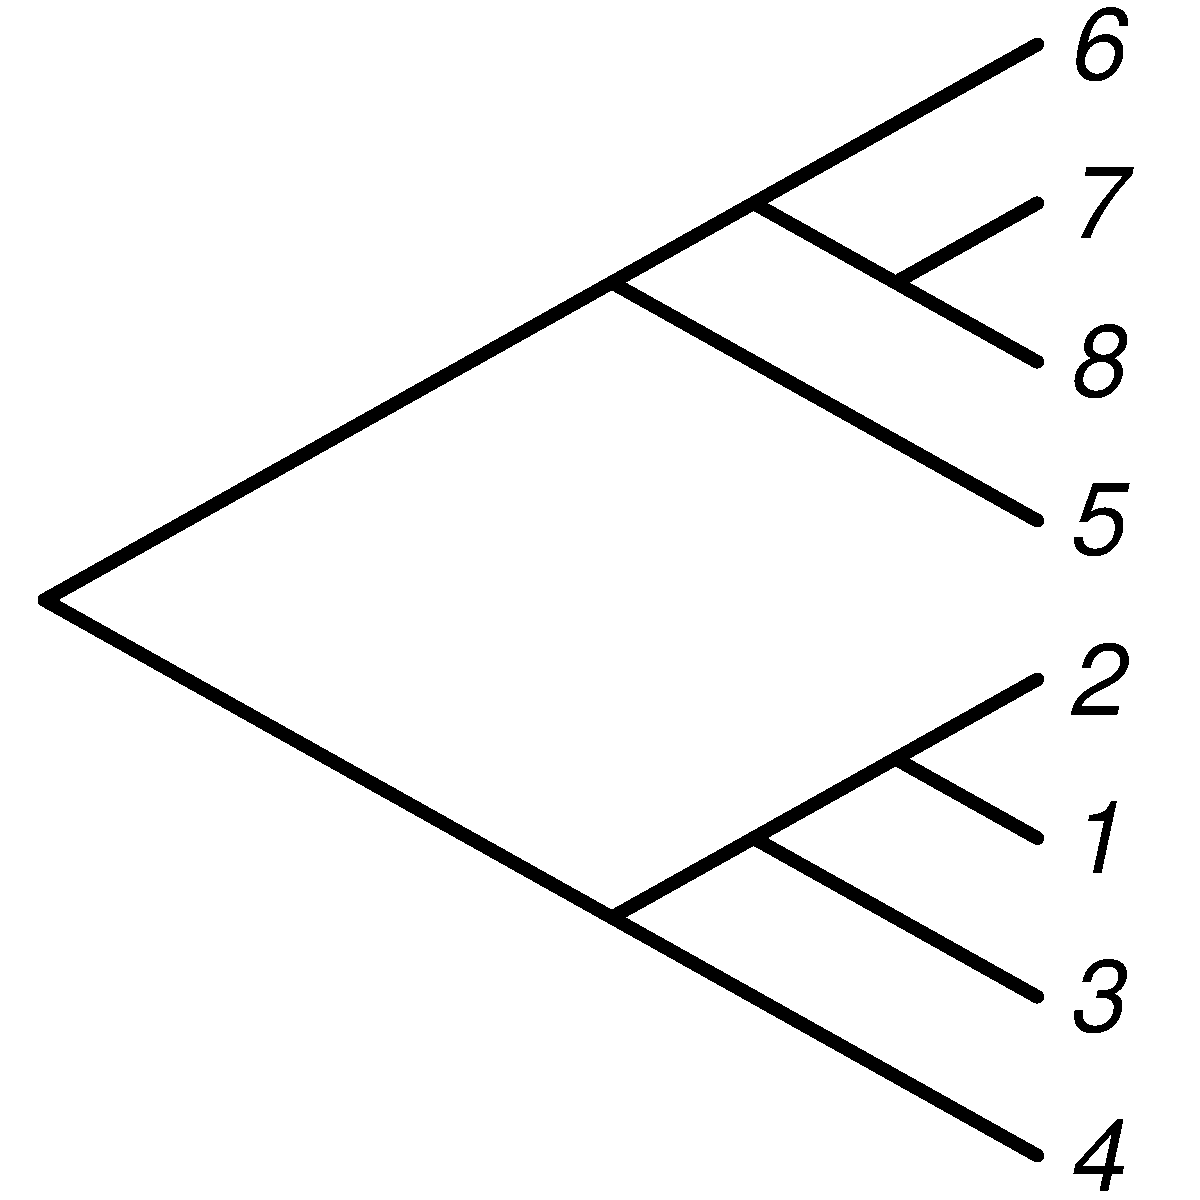
\includegraphics[width=.95\linewidth]{gatk_tree_rightwards.pdf} & 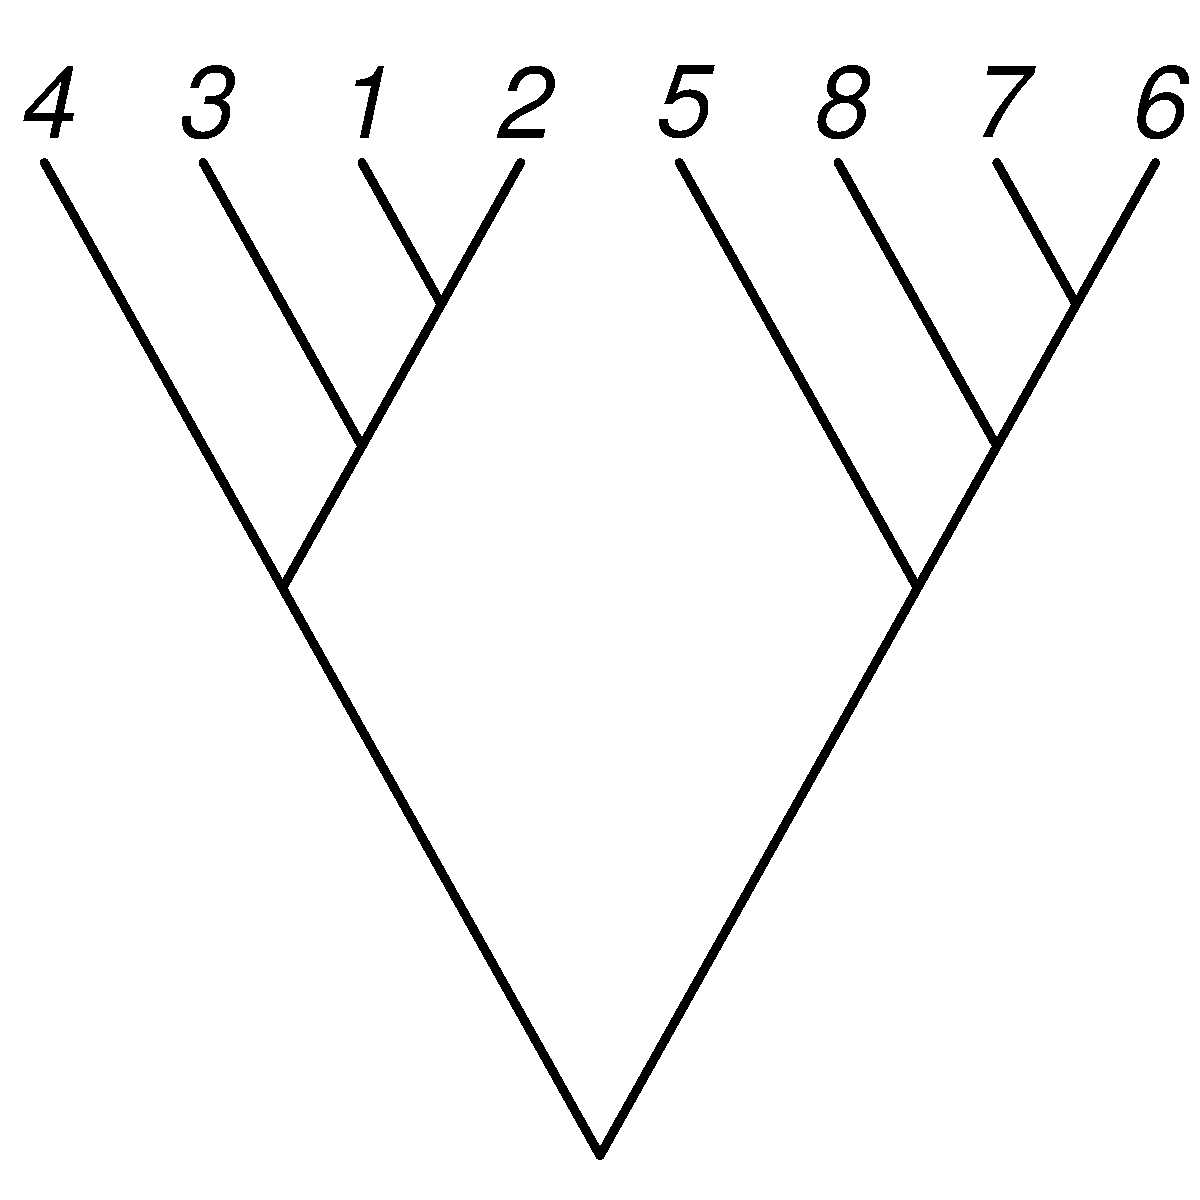
\includegraphics[width=.95\linewidth,angle=90]{true_tree.pdf} \\
%   & & \\
%  DiscoSNP++ & 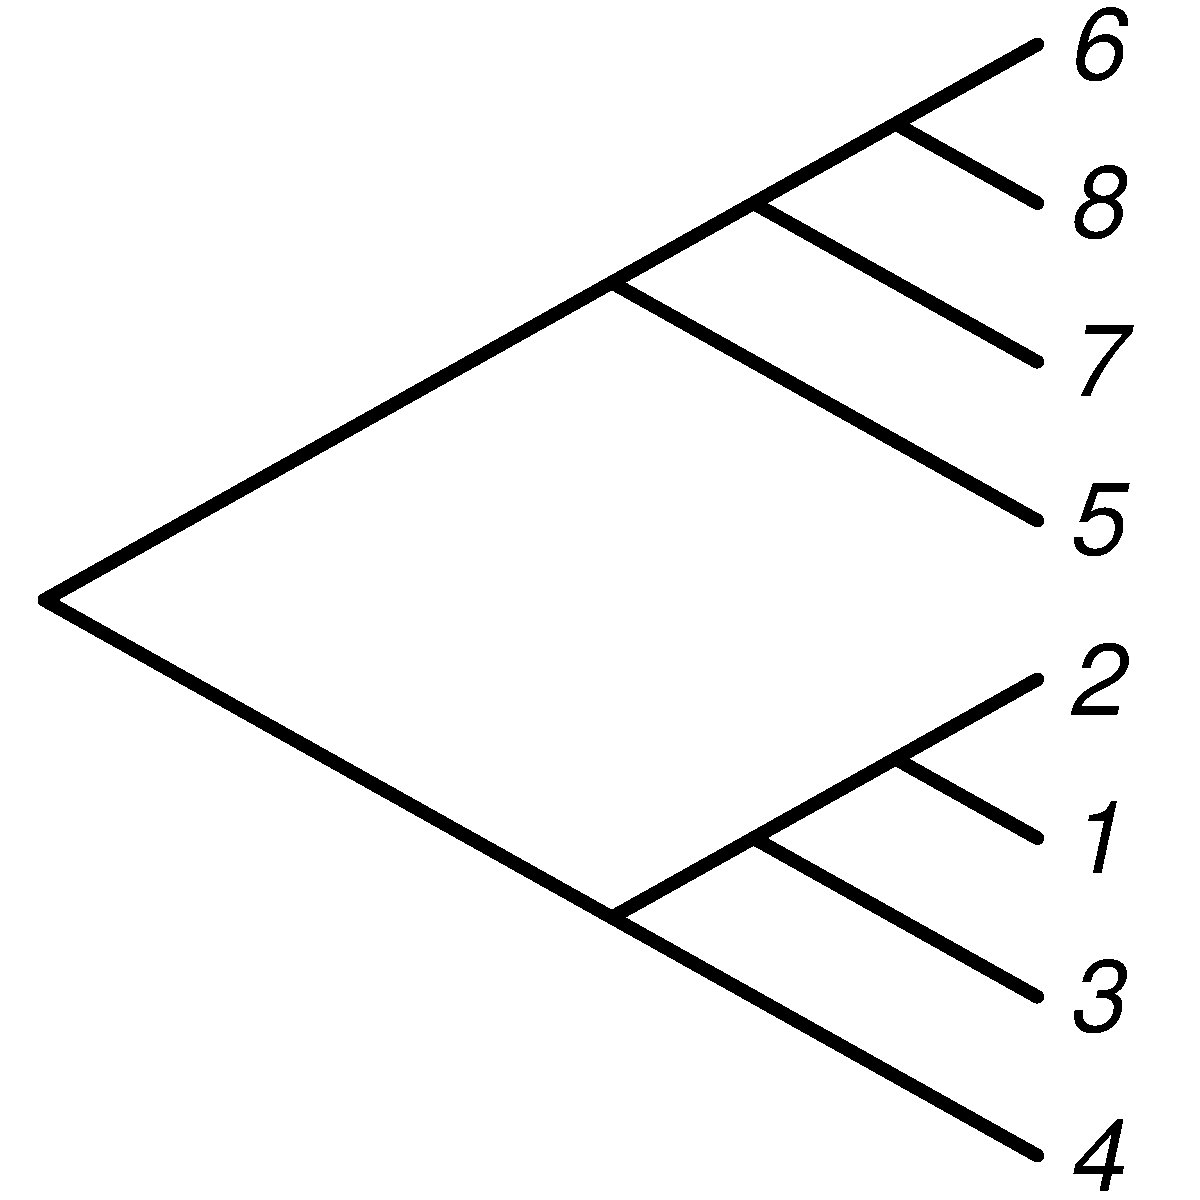
\includegraphics[width=.95\linewidth]{disco_tree_rightwards.pdf} & 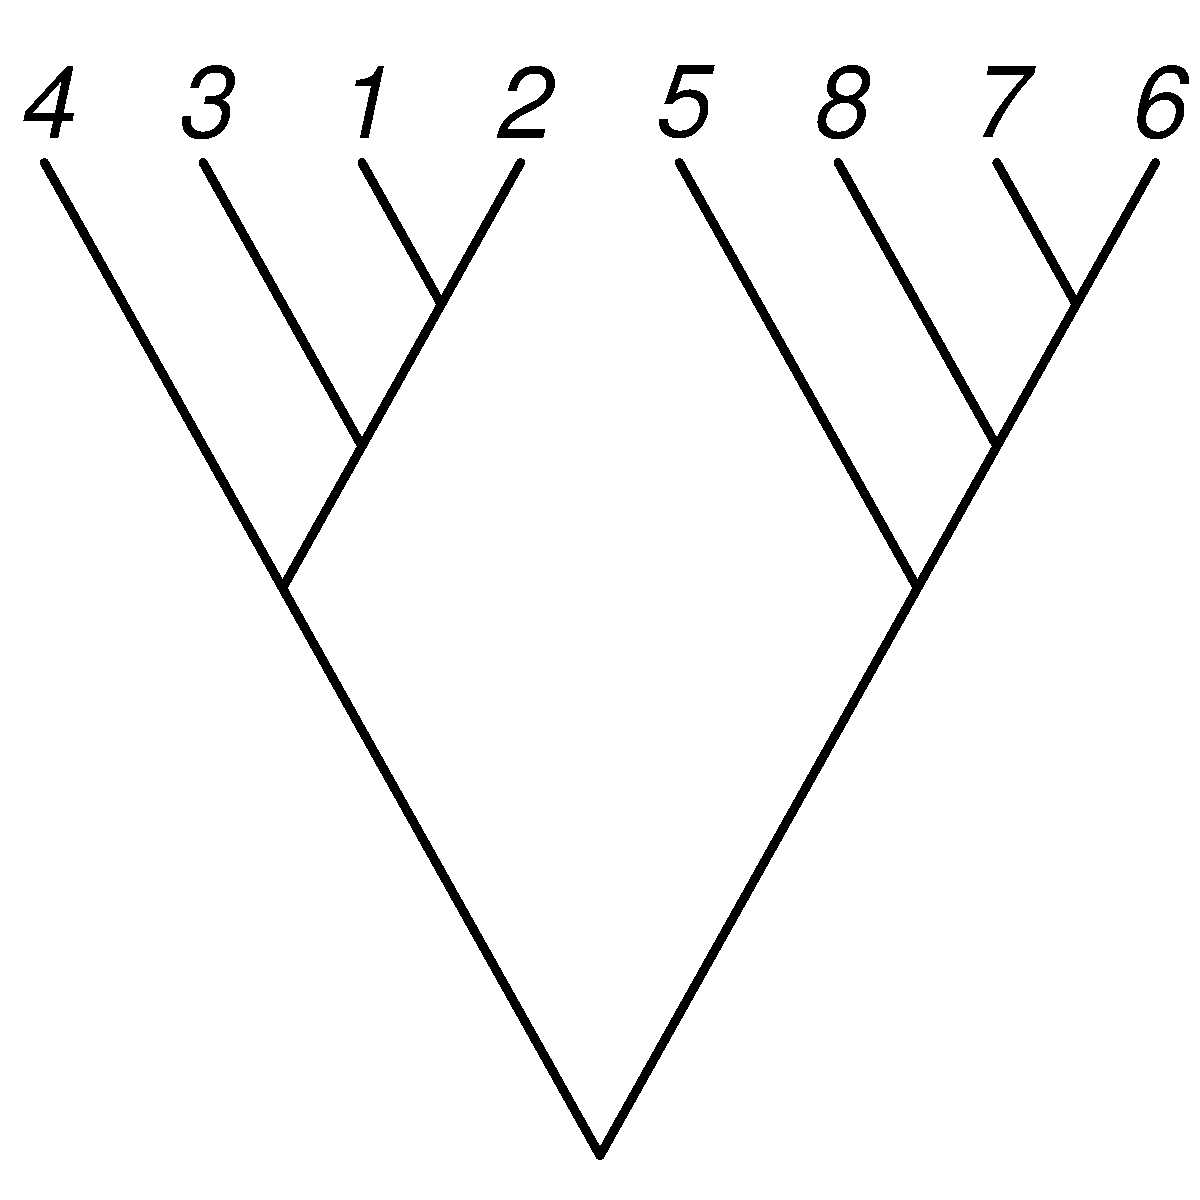
\includegraphics[width=.95\linewidth,angle=90]{true_tree.pdf}
% \end{tabu}
% \end{center}

% % \vskip 3ex

% % \begin{itemize}
% % \item The toplogy of the tree built from variants called by reference-free method DiscoSNP++ closely resembles the branching pattern of the plant.
% % \vskip 1ex
% % \item DiscoSNP++ performance matches that of GATK used with a reference from the closely-related species \textit{Eucalyptus grandis}.
% % \vskip 1ex
% % \item A short internode causes incorrect placement of branches 6, 7, and 8 for both methods.
% % \end{itemize}

% \end{block}



% %%% Right Side %%%%

\column{.5\linewidth}

\begin{block}{Quality Score Significance}
\begin{center}
\begin{tabular}{ c | c | c }
\bfseries Quality Score & \bfseries Illumina Bin & \bfseries $P(error)$ \\
\hline
1 & N &  0.8 \\
2 & 6 &  0.6 \\
3 & 6 &  0.5 \\
4 & 6 &  0.4 \\
5 & 6 &  0.3 \\
6 & 6 &  0.3 \\
7 & 6 &  0.2 \\
8 & 6 &  0.2 \\
9 & 6 &  0.1 \\
\bfseries 10 & \bfseries 15 & \bfseries  0.1 \\
11 & 15 & 0.08 \\
12 & 15 & 0.06 \\
13 & 15 & 0.05 \\
14 & 15 & 0.04 \\
15 & 15 & 0.03 \\
16 & 15 & 0.03 \\
17 & 15 & 0.02 \\
18 & 15 & 0.02 \\
19 & 15 & 0.01 \\
\bfseries 20 & \bfseries 27 & \bfseries 0.01 \\
\bfseries 30 & \bfseries 33 & \bfseries 0.001 \\
\bfseries 40 & \bfseries 40 & \bfseries 0.0001 \\

\end{tabular}
\end{center}
\end{block}

% %%%%%%%%%%%%%%%%%%%

% \begin{block}{Next steps: Reference Improvement}

% We improve our reference by aligning to the \textit{E. grandis} genome, then creating a consensus from that alignment. This can be repeated until convergence.

% \vskip 1ex

% \begin{center}
% 	\begin{tikzpicture}[cnode/.style={rectangle,draw=black!60,fill=black!5,very thick}, node distance = 3 cm]
% 		\node[cnode] (reads){Reads};
% 		\node[cnode] (eg)[below = .5cm of reads]{\textit{E. grandis}};
% 		\node[cnode] (em1)[right = of eg]{\textit{E. melliodora} 1};
% 		\node[cnode] (em2)[right = of em1]{\textit{E. melliodora} 2};
% 		\node[cnode] (etc)[right = of em2] {...};
% 		\draw[line width=3mm,->] ($(reads.east)-(0cm,.5cm)$) -- ($(reads.east)+(2cm,-.5cm)$) |- (em1.west);
% 		\draw[line width=3mm,->] (reads.east) -- ($(reads.east)+(13cm,0cm)$) |- (em2.west);
% 		\draw[line width=3mm,->] ($(reads.east)+(0cm,.5cm)$) -- ($(reads.east)+(24cm,.5cm)$) |- (etc.west);
% 		\draw[line width=3mm,->] (eg) -- (em1);
% 		\draw[line width=3mm,->] (em1) -- (em2);
% 		\draw[line width=3mm,->] (em2) -- (etc);
% 	\end{tikzpicture}
% \end{center}

% \end{block}


% \begin{block}{Results: Iterative Mapping Improves Reference}

% \begin{center}
% 	\begin{tikzpicture}[align=center,cnode/.style={rectangle,draw=black!60,fill=black!5,very thick}, node distance = .5cm and 2.5 cm]
% 		\node[cnode] (reads){Reads};
% 		\node[cnode] (eg)[below = of reads]{\textit{E. grandis}};
% 		\node[cnode] (em1)[right = of eg]{\textit{E. melliodora} 1};
% 		\node[cnode] (em1q)[right = of em1]{Alignment Quality Scores};
% 		\node[cnode] (egq)[below = of em1q]{Alignment Quality Scores};
% 		\draw[line width=3mm,->] ($(reads.east)-(0cm,.25cm)$) -- ($(reads.east)+(1.5cm,-.25cm)$) |- (em1.west);
% 		\draw[line width=3mm,->] ($(eg.east)+(1.25cm,0cm)$) -- ($(eg.east)+(1.25cm,-1cm)$) |- (egq.west);
% 		\draw[line width=3mm,->] (eg) -- (em1);
% 		\draw[line width=3mm,->] (em1) -- (em1q);
% 		\draw[line width=3mm,->] ($(reads.east)+(0cm,.25cm)$) -- ($(reads.east)+(12.5cm,.25cm)$) |- (em1q.west);
% 	\end{tikzpicture}
% \end{center}

% \vskip 1ex

% \begin{center}

% 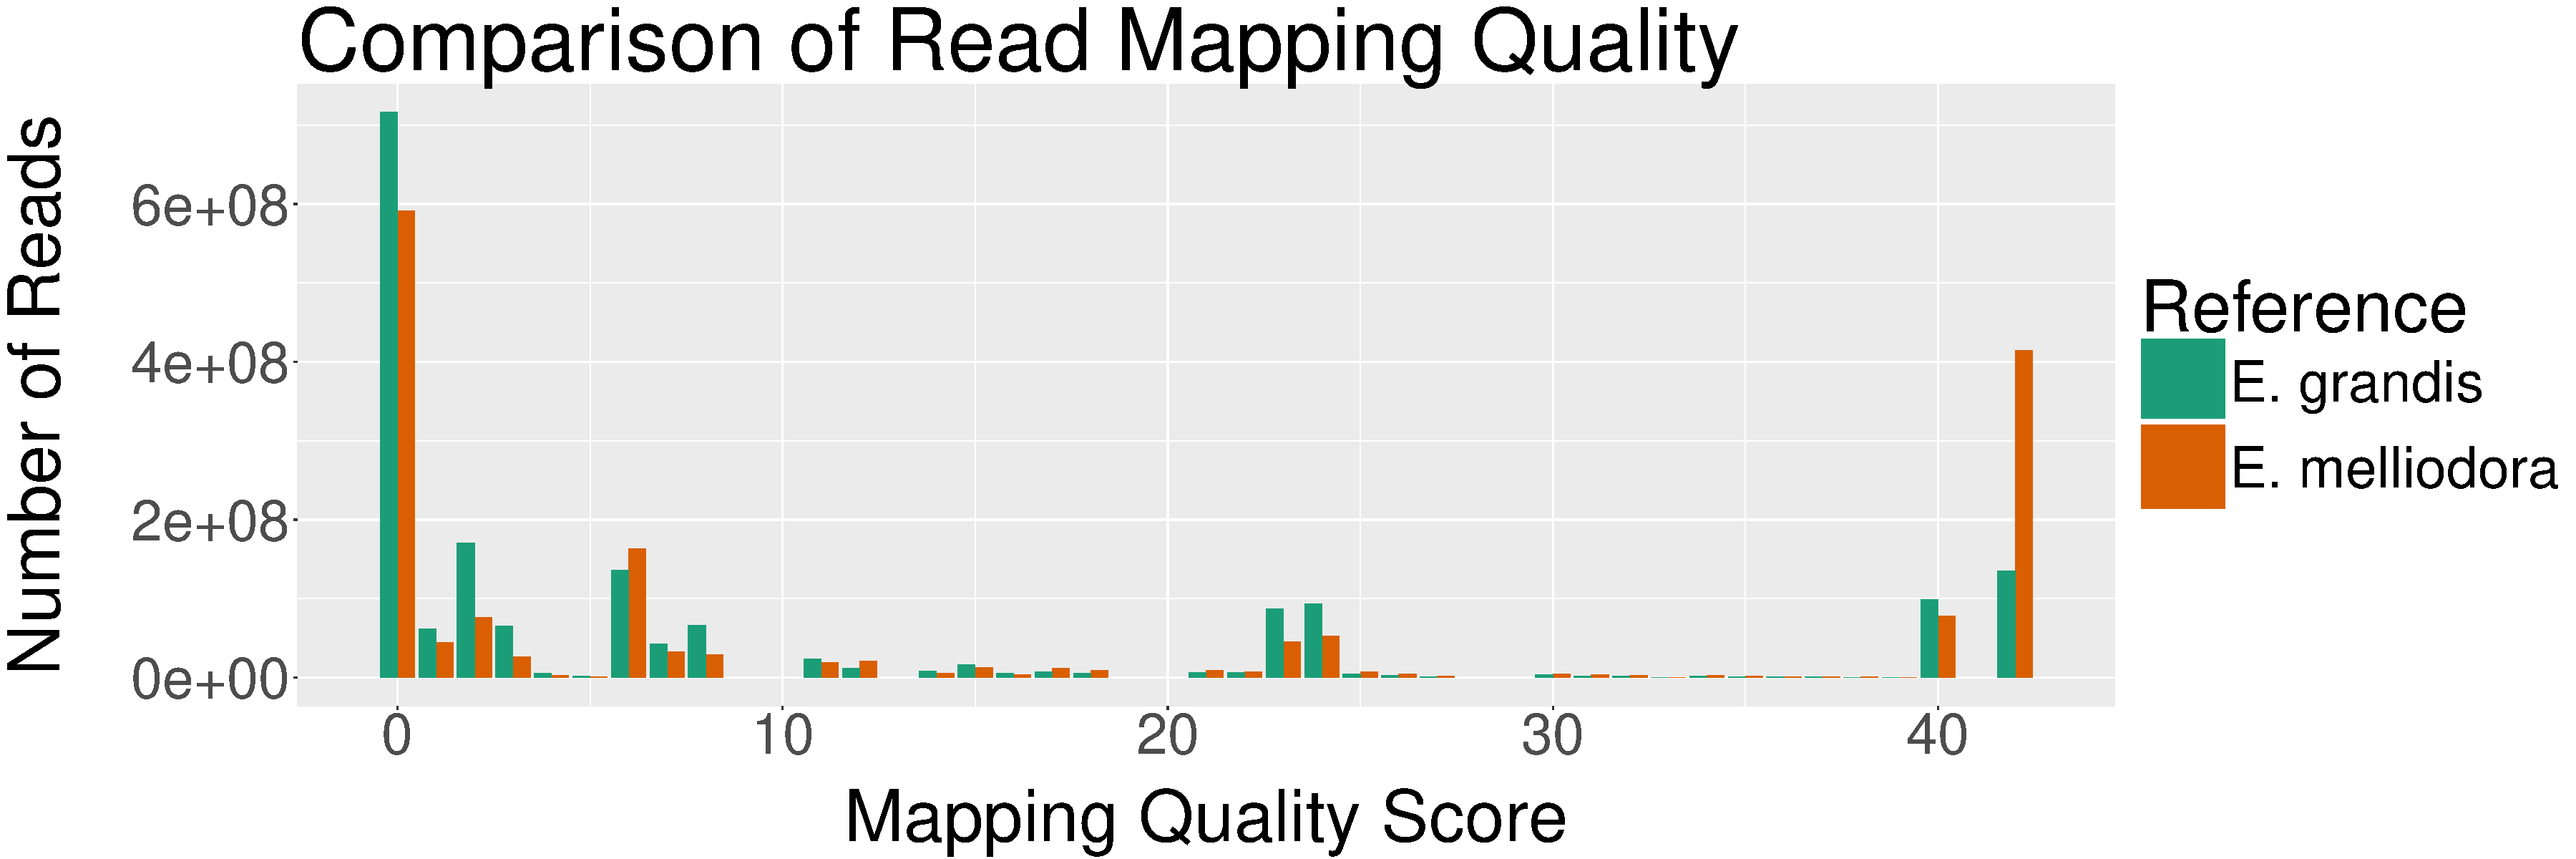
\includegraphics[width=.95\linewidth]{both_hist.pdf}

% \end{center}

% % \vskip 1ex

% Alignment to the consensus sequence produces an alignment with higher overall quality scores than alignment to the \textit{Eucalyptus grandis} reference.

% \end{block}


% \begin{block}{Results: Aligner Choice Affects Generated Reference Quality}

% \begin{center}
% 	\begin{tikzpicture}[align=center,cnode/.style={rectangle,draw=black!60,fill=black!5,very thick}, node distance = 2cm and 2cm]
% 		\node[cnode] (eg){\textit{E. grandis}};
% 		\node[cnode,minimum width=11cm] (reads)[right = of eg]{Reads};
% 		\node[cnode] (em1)[above right = 2cm and 4cm of eg]{\textit{E. melliodora} 1};
% 		\node[cnode] (em2)[below right = 2cm and 4cm of eg]{\textit{E. melliodora} 1};
% 		\node[cnode] (bwaq)[right = 4cm of em1]{Quality Scores};
% 		\node[cnode] (ngmq)[right = 4cm of em2]{Quality Scores};
% 		\draw[line width=3mm,->] (eg.north) |- (em1);
% 		\draw[line width=3mm,->] (eg.south) |- (em2);
% 		% \draw[line width=3mm,->] ($(reads.west)+(0cm,.5cm)$) to[out=180,in=180] ($(em1.west)-(1.5cm,0cm)$) -- (em1.west);
% 		\draw[line width=3mm,->] ($(reads.west)+(0cm,.5cm)$) -- ++(-1cm,0cm) |- (em1.west) node[pos=.25,right]{BWA};
% 		\draw[line width=3mm,->] ($(reads.west)-(0cm,.5cm)$) -- ++(-1cm,0cm) |- (em2.west) node[pos=.25,right]{NGM};
% 		\draw[line width=3mm,->] (em1) -- (bwaq);
% 		\draw[line width=3mm,->] (em2) -- (ngmq);
% 		\draw[line width=3mm,->] ($(reads.east)+(0cm,.5cm)$) -- ++(1cm,0cm) |- (bwaq.west) node[pos=.2,right]{Bowtie};
% 		\draw[line width=3mm,->] ($(reads.east)-(0cm,.5cm)$) -- ++(1cm,0cm) |- (ngmq.west) node[pos=.2,right]{Bowtie};
% 	\end{tikzpicture}
% \end{center}

% \vskip 1ex

% \begin{center}

% 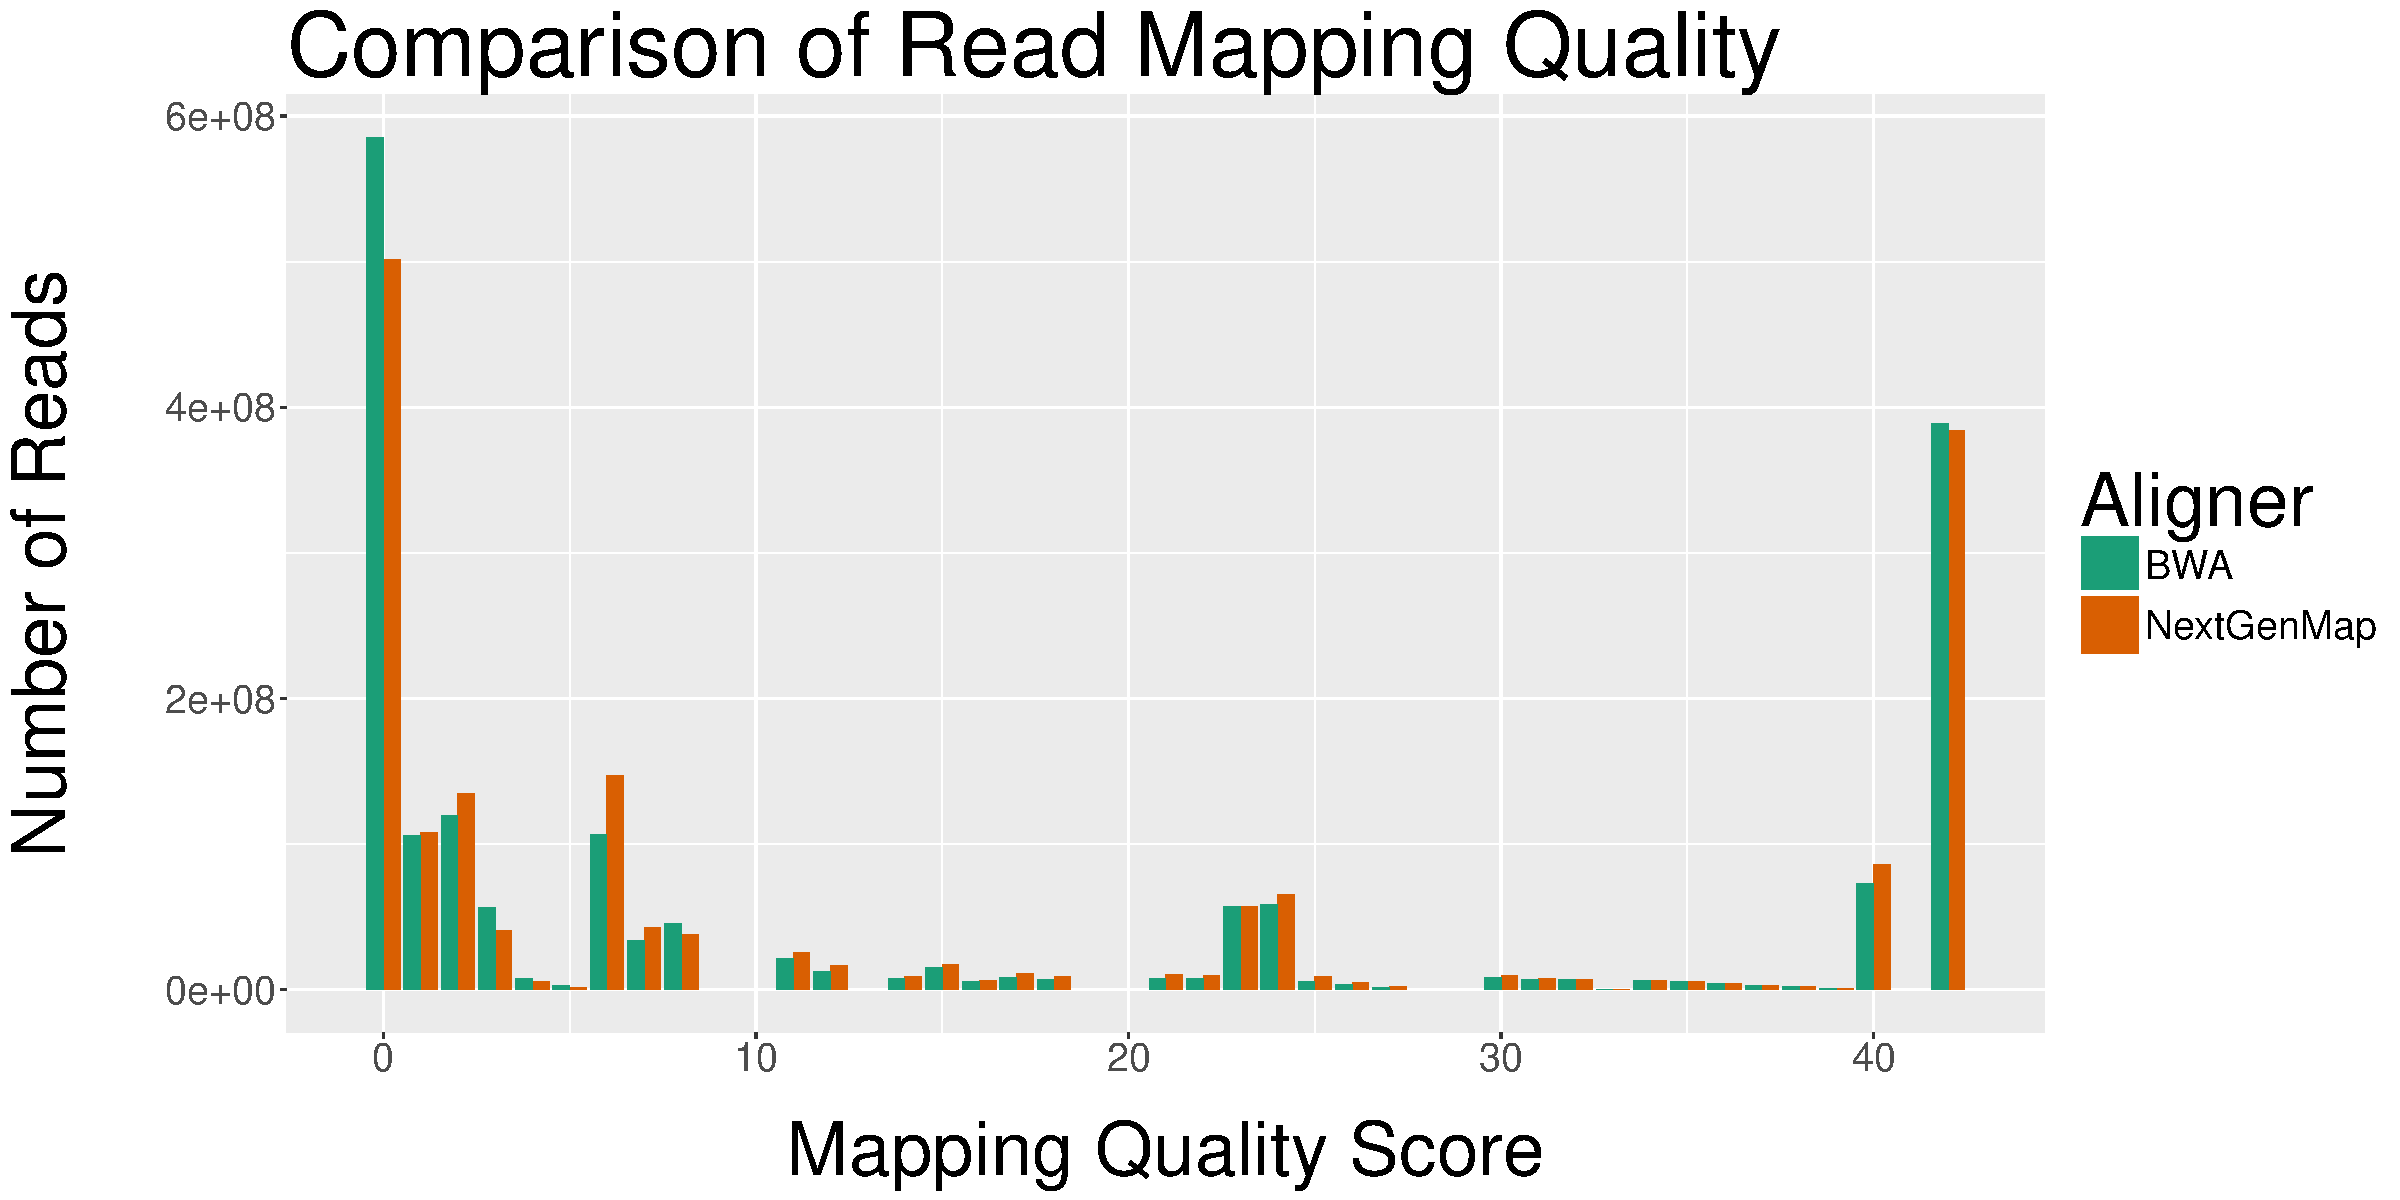
\includegraphics[width=.95\linewidth]{aligner_comparison_hist.pdf}

% \end{center}

% % \vskip 1ex

% % A reference created from a NextGenMap alignment produces less unmapped reads than one created from a BWA alignment.

% \end{block}




% \begin{block}{Conclusions}

% \begin{itemize}
% 	\item Phylogenies of somatic mutations within a \textit{Eucalyptus} tree match the branching patterns of the tree using both a reference-based and a reference-free variant caller.
% 	\item Aligning reads to a close relative, obtaining a consensus sequence, then realigning to that consensus seems to improve alignment quality.
% \end{itemize}

% \end{block}

\begin{block}{Next Steps}
\begin{itemize}
	\item Test performance against GATK BQSR with varying levels of false positives and false negatives.
	\item Simulate reads from a distant genome and compare performance with GATK BQSR.
	\item Linear model improvements
	\item Programming optimizations.
\end{itemize}
\end{block}


\begin{block}{Software}

\faicon{github} \url{https://github.com/adamjorr/kbbq}

\end{block}

\begin{block}{Acknowledgements}

% \begin{center}

\begin{columns}
%\column{.4\linewidth}
%This work is supported by grants NIH R01-HG007178 and NSF DBI-1356548.
\column{.27\linewidth}

\includegraphics[width=\linewidth]{lab_logo.pdf}
\column{.27\linewidth}

\includegraphics[width=\linewidth]{sols_logo.pdf}
\column{.3\linewidth}

\includegraphics[width=\linewidth]{biodesign_logo.pdf}
\end{columns}

% \end{center}

\end{block}

\end{columns}
\end{frame}

\end{document}